\begin{figure}[h!]
	\centering
	
	
	
	
	\tikzset{every picture/.style={line width=0.75pt}} %set default line width to 0.75pt        
	
	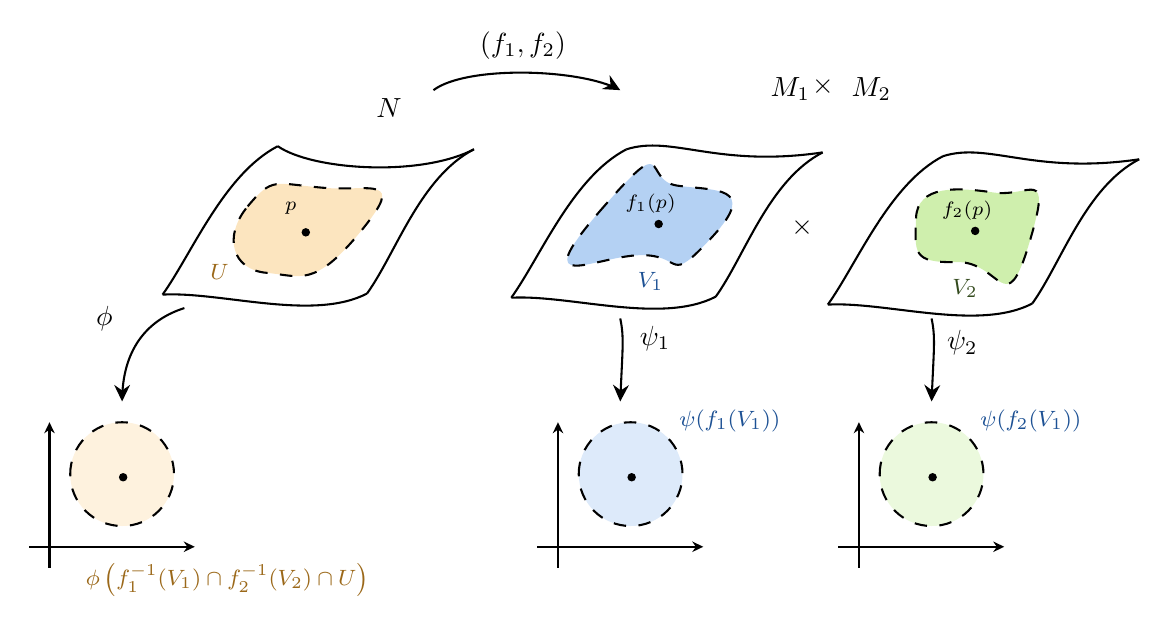
\begin{tikzpicture}[x=0.75pt,y=0.75pt,yscale=-1,xscale=1]
		%uncomment if require: \path (0,300); %set diagram left start at 0, and has height of 300
		
		%Curve Lines [id:da10777202147976128] 
		\draw    (89.5,138.5) .. controls (103.5,119) and (119,80.5) .. (145,67) ;
		%Curve Lines [id:da9226409814736687] 
		\draw    (89.5,138.5) .. controls (118,137) and (162,151.5) .. (188,138) ;
		%Curve Lines [id:da6153501766442295] 
		\draw    (188,138) .. controls (202,118.5) and (213.5,82) .. (239.5,68.5) ;
		%Curve Lines [id:da8299437341096081] 
		\draw    (145,67) .. controls (161.5,78.5) and (213.5,82) .. (239.5,68.5) ;
		%Curve Lines [id:da708998797665932] 
		\draw    (257.5,140) .. controls (271.5,120.5) and (287,82) .. (313,68.5) ;
		%Curve Lines [id:da5763078865113123] 
		\draw    (257.5,140) .. controls (286,138.5) and (330,153) .. (356,139.5) ;
		%Curve Lines [id:da17448723811544053] 
		\draw    (356,139.5) .. controls (370,120) and (381.5,83.5) .. (407.5,70) ;
		%Curve Lines [id:da5843329628503129] 
		\draw    (313,68.5) .. controls (335,61.5) and (356.5,77.5) .. (407.5,70) ;
		%Shape: Polygon Curved [id:ds719249129813768] 
		\draw  [fill={rgb, 255:red, 245; green, 166; blue, 35 }  ,fill opacity=0.29 ][dash pattern={on 4.5pt off 4.5pt}] (130.5,96) .. controls (142.5,81.5) and (143.5,85) .. (166.5,87) .. controls (189.5,89) and (207.5,80.5) .. (185,108) .. controls (162.5,135.5) and (156,129.5) .. (139.5,128) .. controls (123,126.5) and (118.5,110.5) .. (130.5,96) -- cycle ;
		%Shape: Polygon Curved [id:ds20297397591709365] 
		\draw  [fill={rgb, 255:red, 74; green, 144; blue, 226 }  ,fill opacity=0.41 ][dash pattern={on 4.5pt off 4.5pt}] (300,98.5) .. controls (335.5,57.5) and (320,83.5) .. (337.5,86) .. controls (355,88.5) and (377,86) .. (354.5,110.5) .. controls (332,135) and (341,119) .. (319.5,119.5) .. controls (298,120) and (264.5,139.5) .. (300,98.5) -- cycle ;
		%Straight Lines [id:da8177031700071737] 
		\draw    (35,203) -- (35,270) ;
		\draw [shift={(35,200)}, rotate = 90] [fill={rgb, 255:red, 0; green, 0; blue, 0 }  ][line width=0.08]  [draw opacity=0] (5.36,-2.57) -- (0,0) -- (5.36,2.57) -- (3.56,0) -- cycle    ;
		%Straight Lines [id:da5847590524068735] 
		\draw    (102,260) -- (25,260) ;
		\draw [shift={(105,260)}, rotate = 180] [fill={rgb, 255:red, 0; green, 0; blue, 0 }  ][line width=0.08]  [draw opacity=0] (5.36,-2.57) -- (0,0) -- (5.36,2.57) -- (3.56,0) -- cycle    ;
		%Shape: Circle [id:dp5757945587417739] 
		\draw  [fill={rgb, 255:red, 245; green, 166; blue, 35 }  ,fill opacity=0.15 ][dash pattern={on 4.5pt off 4.5pt}] (45,225) .. controls (45,211.19) and (56.19,200) .. (70,200) .. controls (83.81,200) and (95,211.19) .. (95,225) .. controls (95,238.81) and (83.81,250) .. (70,250) .. controls (56.19,250) and (45,238.81) .. (45,225) -- cycle ;
		%Straight Lines [id:da9243110317223102] 
		\draw    (280,203) -- (280,270) ;
		\draw [shift={(280,200)}, rotate = 90] [fill={rgb, 255:red, 0; green, 0; blue, 0 }  ][line width=0.08]  [draw opacity=0] (5.36,-2.57) -- (0,0) -- (5.36,2.57) -- (3.56,0) -- cycle    ;
		%Straight Lines [id:da35917271861832445] 
		\draw    (347,260) -- (270,260) ;
		\draw [shift={(350,260)}, rotate = 180] [fill={rgb, 255:red, 0; green, 0; blue, 0 }  ][line width=0.08]  [draw opacity=0] (5.36,-2.57) -- (0,0) -- (5.36,2.57) -- (3.56,0) -- cycle    ;
		%Shape: Circle [id:dp7567118959752777] 
		\draw  [fill={rgb, 255:red, 74; green, 144; blue, 226 }  ,fill opacity=0.19 ][dash pattern={on 4.5pt off 4.5pt}] (290,225) .. controls (290,211.19) and (301.19,200) .. (315,200) .. controls (328.81,200) and (340,211.19) .. (340,225) .. controls (340,238.81) and (328.81,250) .. (315,250) .. controls (301.19,250) and (290,238.81) .. (290,225) -- cycle ;
		%Curve Lines [id:da8387568355499948] 
		\draw    (220,40) .. controls (235.36,28.48) and (286.66,29.4) .. (307.55,38.78) ;
		\draw [shift={(310,40)}, rotate = 208.93] [fill={rgb, 255:red, 0; green, 0; blue, 0 }  ][line width=0.08]  [draw opacity=0] (8.04,-3.86) -- (0,0) -- (8.04,3.86) -- (5.34,0) -- cycle    ;
		%Curve Lines [id:da5596780294001671] 
		\draw    (310,150) .. controls (311.92,159.12) and (311.08,164.55) .. (310.12,187.09) ;
		\draw [shift={(310,190)}, rotate = 272.29] [fill={rgb, 255:red, 0; green, 0; blue, 0 }  ][line width=0.08]  [draw opacity=0] (8.04,-3.86) -- (0,0) -- (8.04,3.86) -- (5.34,0) -- cycle    ;
		%Curve Lines [id:da33319736118491083] 
		\draw    (100,145) .. controls (83.11,150.31) and (70.88,163.53) .. (70.05,187.36) ;
		\draw [shift={(70,190)}, rotate = 270] [fill={rgb, 255:red, 0; green, 0; blue, 0 }  ][line width=0.08]  [draw opacity=0] (8.04,-3.86) -- (0,0) -- (8.04,3.86) -- (5.34,0) -- cycle    ;
		%Shape: Circle [id:dp912491598557873] 
		\draw  [fill={rgb, 255:red, 0; green, 0; blue, 0 }  ,fill opacity=1 ] (157,108.5) .. controls (157,107.67) and (157.67,107) .. (158.5,107) .. controls (159.33,107) and (160,107.67) .. (160,108.5) .. controls (160,109.33) and (159.33,110) .. (158.5,110) .. controls (157.67,110) and (157,109.33) .. (157,108.5) -- cycle ;
		%Shape: Circle [id:dp5874182665613439] 
		\draw  [fill={rgb, 255:red, 0; green, 0; blue, 0 }  ,fill opacity=1 ] (327,104.5) .. controls (327,103.67) and (327.67,103) .. (328.5,103) .. controls (329.33,103) and (330,103.67) .. (330,104.5) .. controls (330,105.33) and (329.33,106) .. (328.5,106) .. controls (327.67,106) and (327,105.33) .. (327,104.5) -- cycle ;
		%Shape: Circle [id:dp6918787727605586] 
		\draw  [fill={rgb, 255:red, 0; green, 0; blue, 0 }  ,fill opacity=1 ] (69,226.5) .. controls (69,225.67) and (69.67,225) .. (70.5,225) .. controls (71.33,225) and (72,225.67) .. (72,226.5) .. controls (72,227.33) and (71.33,228) .. (70.5,228) .. controls (69.67,228) and (69,227.33) .. (69,226.5) -- cycle ;
		%Shape: Circle [id:dp5802827719353891] 
		\draw  [fill={rgb, 255:red, 0; green, 0; blue, 0 }  ,fill opacity=1 ] (314,226.5) .. controls (314,225.67) and (314.67,225) .. (315.5,225) .. controls (316.33,225) and (317,225.67) .. (317,226.5) .. controls (317,227.33) and (316.33,228) .. (315.5,228) .. controls (314.67,228) and (314,227.33) .. (314,226.5) -- cycle ;
		%Curve Lines [id:da5866172687533027] 
		\draw    (410,143.32) .. controls (424,123.82) and (439.5,85.32) .. (465.5,71.82) ;
		%Curve Lines [id:da33769380232352386] 
		\draw    (410,143.32) .. controls (438.5,141.82) and (482.5,156.32) .. (508.5,142.82) ;
		%Curve Lines [id:da5667601010223242] 
		\draw    (508.5,142.82) .. controls (522.5,123.32) and (534,86.82) .. (560,73.32) ;
		%Curve Lines [id:da7766245611502776] 
		\draw    (465.5,71.82) .. controls (487.5,64.82) and (509,80.82) .. (560,73.32) ;
		%Shape: Polygon Curved [id:ds9848033990053162] 
		\draw  [fill={rgb, 255:red, 126; green, 211; blue, 33 }  ,fill opacity=0.37 ][dash pattern={on 4.5pt off 4.5pt}] (452.5,101.82) .. controls (453,85.5) and (472.5,86.82) .. (490,89.32) .. controls (507.5,91.82) and (518.5,75.5) .. (507,113.82) .. controls (495.5,152.14) and (493.5,122.32) .. (472,122.82) .. controls (450.5,123.32) and (452,118.14) .. (452.5,101.82) -- cycle ;
		%Shape: Circle [id:dp8441479070293367] 
		\draw  [fill={rgb, 255:red, 0; green, 0; blue, 0 }  ,fill opacity=1 ] (479.5,107.82) .. controls (479.5,106.99) and (480.17,106.32) .. (481,106.32) .. controls (481.83,106.32) and (482.5,106.99) .. (482.5,107.82) .. controls (482.5,108.65) and (481.83,109.32) .. (481,109.32) .. controls (480.17,109.32) and (479.5,108.65) .. (479.5,107.82) -- cycle ;
		%Straight Lines [id:da4245600664130684] 
		\draw    (425,203) -- (425,270) ;
		\draw [shift={(425,200)}, rotate = 90] [fill={rgb, 255:red, 0; green, 0; blue, 0 }  ][line width=0.08]  [draw opacity=0] (5.36,-2.57) -- (0,0) -- (5.36,2.57) -- (3.56,0) -- cycle    ;
		%Straight Lines [id:da8383634096867163] 
		\draw    (492,260) -- (415,260) ;
		\draw [shift={(495,260)}, rotate = 180] [fill={rgb, 255:red, 0; green, 0; blue, 0 }  ][line width=0.08]  [draw opacity=0] (5.36,-2.57) -- (0,0) -- (5.36,2.57) -- (3.56,0) -- cycle    ;
		%Shape: Circle [id:dp032856070596776865] 
		\draw  [fill={rgb, 255:red, 184; green, 233; blue, 134 }  ,fill opacity=0.28 ][dash pattern={on 4.5pt off 4.5pt}] (435,225) .. controls (435,211.19) and (446.19,200) .. (460,200) .. controls (473.81,200) and (485,211.19) .. (485,225) .. controls (485,238.81) and (473.81,250) .. (460,250) .. controls (446.19,250) and (435,238.81) .. (435,225) -- cycle ;
		%Shape: Circle [id:dp2655157582176253] 
		\draw  [fill={rgb, 255:red, 0; green, 0; blue, 0 }  ,fill opacity=1 ] (459,226.5) .. controls (459,225.67) and (459.67,225) .. (460.5,225) .. controls (461.33,225) and (462,225.67) .. (462,226.5) .. controls (462,227.33) and (461.33,228) .. (460.5,228) .. controls (459.67,228) and (459,227.33) .. (459,226.5) -- cycle ;
		%Curve Lines [id:da36500972985566005] 
		\draw    (460,150) .. controls (461.92,159.12) and (461.08,164.55) .. (460.12,187.09) ;
		\draw [shift={(460,190)}, rotate = 272.29] [fill={rgb, 255:red, 0; green, 0; blue, 0 }  ][line width=0.08]  [draw opacity=0] (8.04,-3.86) -- (0,0) -- (8.04,3.86) -- (5.34,0) -- cycle    ;
		
		% Text Node
		\draw (191,42.4) node [anchor=north west][inner sep=0.75pt]    {$N$};
		% Text Node
		\draw (381,32.4) node [anchor=north west][inner sep=0.75pt]    {$M_{1}$};
		% Text Node
		\draw (241,10.4) node [anchor=north west][inner sep=0.75pt]    {$( f_{1} ,f_{2})$};
		% Text Node
		\draw (318,152.4) node [anchor=north west][inner sep=0.75pt]    {$\psi _{1}$};
		% Text Node
		\draw (56,142.4) node [anchor=north west][inner sep=0.75pt]    {$\phi $};
		% Text Node
		\draw (147,92.4) node [anchor=north west][inner sep=0.75pt]  [font=\scriptsize]  {$p$};
		% Text Node
		\draw (311,88.4) node [anchor=north west][inner sep=0.75pt]  [font=\scriptsize]  {$f_{1}( p)$};
		% Text Node
		\draw (111,122.4) node [anchor=north west][inner sep=0.75pt]  [font=\footnotesize,color={rgb, 255:red, 155; green, 104; blue, 25 }  ,opacity=1 ]  {$U$};
		% Text Node
		\draw (317,126.4) node [anchor=north west][inner sep=0.75pt]  [font=\footnotesize,color={rgb, 255:red, 29; green, 81; blue, 148 }  ,opacity=1 ]  {$V_{1}$};
		% Text Node
		\draw (337,192.4) node [anchor=north west][inner sep=0.75pt]  [font=\footnotesize,color={rgb, 255:red, 29; green, 81; blue, 148 }  ,opacity=1 ]  {$\psi ( f_{1}( V_{1}))$};
		% Text Node
		\draw (51,266.4) node [anchor=north west][inner sep=0.75pt]  [font=\footnotesize,color={rgb, 255:red, 155; green, 104; blue, 25 }  ,opacity=1 ]  {$\phi \left( f_{1}^{-1}( V_{1}) \cap f_{2}^{-1}( V_{2}) \cap U\right)$};
		% Text Node
		\draw (463.5,91.72) node [anchor=north west][inner sep=0.75pt]  [font=\scriptsize]  {$f_{2}( p)$};
		% Text Node
		\draw (468.5,129.72) node [anchor=north west][inner sep=0.75pt]  [font=\footnotesize,color={rgb, 255:red, 52; green, 75; blue, 30 }  ,opacity=1 ]  {$V_{2}$};
		% Text Node
		\draw (482,192.4) node [anchor=north west][inner sep=0.75pt]  [font=\footnotesize,color={rgb, 255:red, 29; green, 81; blue, 148 }  ,opacity=1 ]  {$\psi ( f_{2}( V_{1}))$};
		% Text Node
		\draw (420,32.4) node [anchor=north west][inner sep=0.75pt]    {$M_{2}$};
		% Text Node
		\draw (391,100.4) node [anchor=north west][inner sep=0.75pt]    {$\times $};
		% Text Node
		\draw (466,154.4) node [anchor=north west][inner sep=0.75pt]    {$\psi _{2}$};
		% Text Node
		\draw (401,32.4) node [anchor=north west][inner sep=0.75pt]    {$\times $};
		
		
	\end{tikzpicture}
\end{figure}